\documentclass{article}
\usepackage[utf8]{inputenc}

\usepackage{authblk}
\usepackage{graphicx}
\graphicspath{{../figures/}}
\usepackage{tabularx}
\usepackage{enumitem}
\usepackage{hyperref}
\usepackage{outlines}
\usepackage{float}
\hypersetup{ 
    colorlinks=true,
    linkcolor=blue,
    filecolor=magenta,      
    urlcolor=cyan,
}

\author[1]{D. Vander-Hyde presenting on behalf of the LHO TCS comissioning team}
\author[2]{LHO TCS commissioning team: T. Vo, D. Brown, G. Mansell, A. Brooks, S. Ballmer, H. Yu, J. Driggers, G. Vajente, H. Yamamoto}


\affil[1,2,5]{Syracuse University}
\affil[3]{University of Adelaide}
\affil[4]{Massachusetts Institute of Technology}
\affil[4,6,7,]{California Institute of Technology}
\affil[1]{dcvander@syr.edu}
\affil[2]{Email id: ba@gmail.com}
\affil[1,3]{Email id: ca@gmail.com}

\title{LHO TCS commissioning for O3}
{
    \makeatletter
    \renewcommand\AB@affilsepx{: \protect\Affilfont}
    \makeatother

    \affil[ ]{Email ids}

    \makeatletter
    \renewcommand\AB@affilsepx{, \protect\Affilfont}
    \makeatother

    \affil[1]{aa@gmail.com}
    \affil[2]{ba@gmail.com}
    \affil[1,3]{ca@gmail.com}
}

\date{March 2019}

\renewcommand{\arraystretch}{1.5}

\begin{document}

\maketitle


\begin{abstract}
%% abstract %%

 The primary role of the currently existing thermal compensation system (TCS) is to probe (via Hartmann wavefront sensors (HWS)) and compensate for (via CO2 lasers and ring heaters) thermo-optic distortions of low spatial frequency that can have potentially adverse affects on mirror geometry which in turn affect interferometer contrast, cavity mode mismatch, reduced cavity buildups, etc. especially when operating at high power. The primary probing is done with Hartmann wavefront sensors placed at each test mass of the dual recycled Fabry-Perot Michelson interferometer and in preparation for O3 we discovered other useful metrics while making final adjustments to TCS actuators. Actuation by negative lensing is performed by a series of installed ring heaters on each of the test masses that form the Fabry Perot cavities while actuation by positive lensing is induced by firing a CO2 laser onto a compensation plate immediately prior to the carrier entering the arm cavity. Relevant measurements and techniques that directly apply to the optimal operation of TCS at the aLIGO Hanford observatory for O3 are detailed. Also discussed are the measurements and effects of point absorbers on input/end test masses. As suggested by models discussed, some of the modeled affects are: higher order mode mismatch from the power recycling cavity to the Y-arm cavity, reduced buildup of RF sidebands in the recycling cavities, and light scatter into higher order modes in the LIGO arm cavities. Keeping the interferometer locked above 30 W input power with the presence of these absorbers is a challenge and may fundamentally limit LHO from achieving a stable configuration at 50 Watts with the currently existing TCS. 
\end{abstract}


\section{Thermal compensation schema for O3}
\begin{figure}[H]
    \centering
        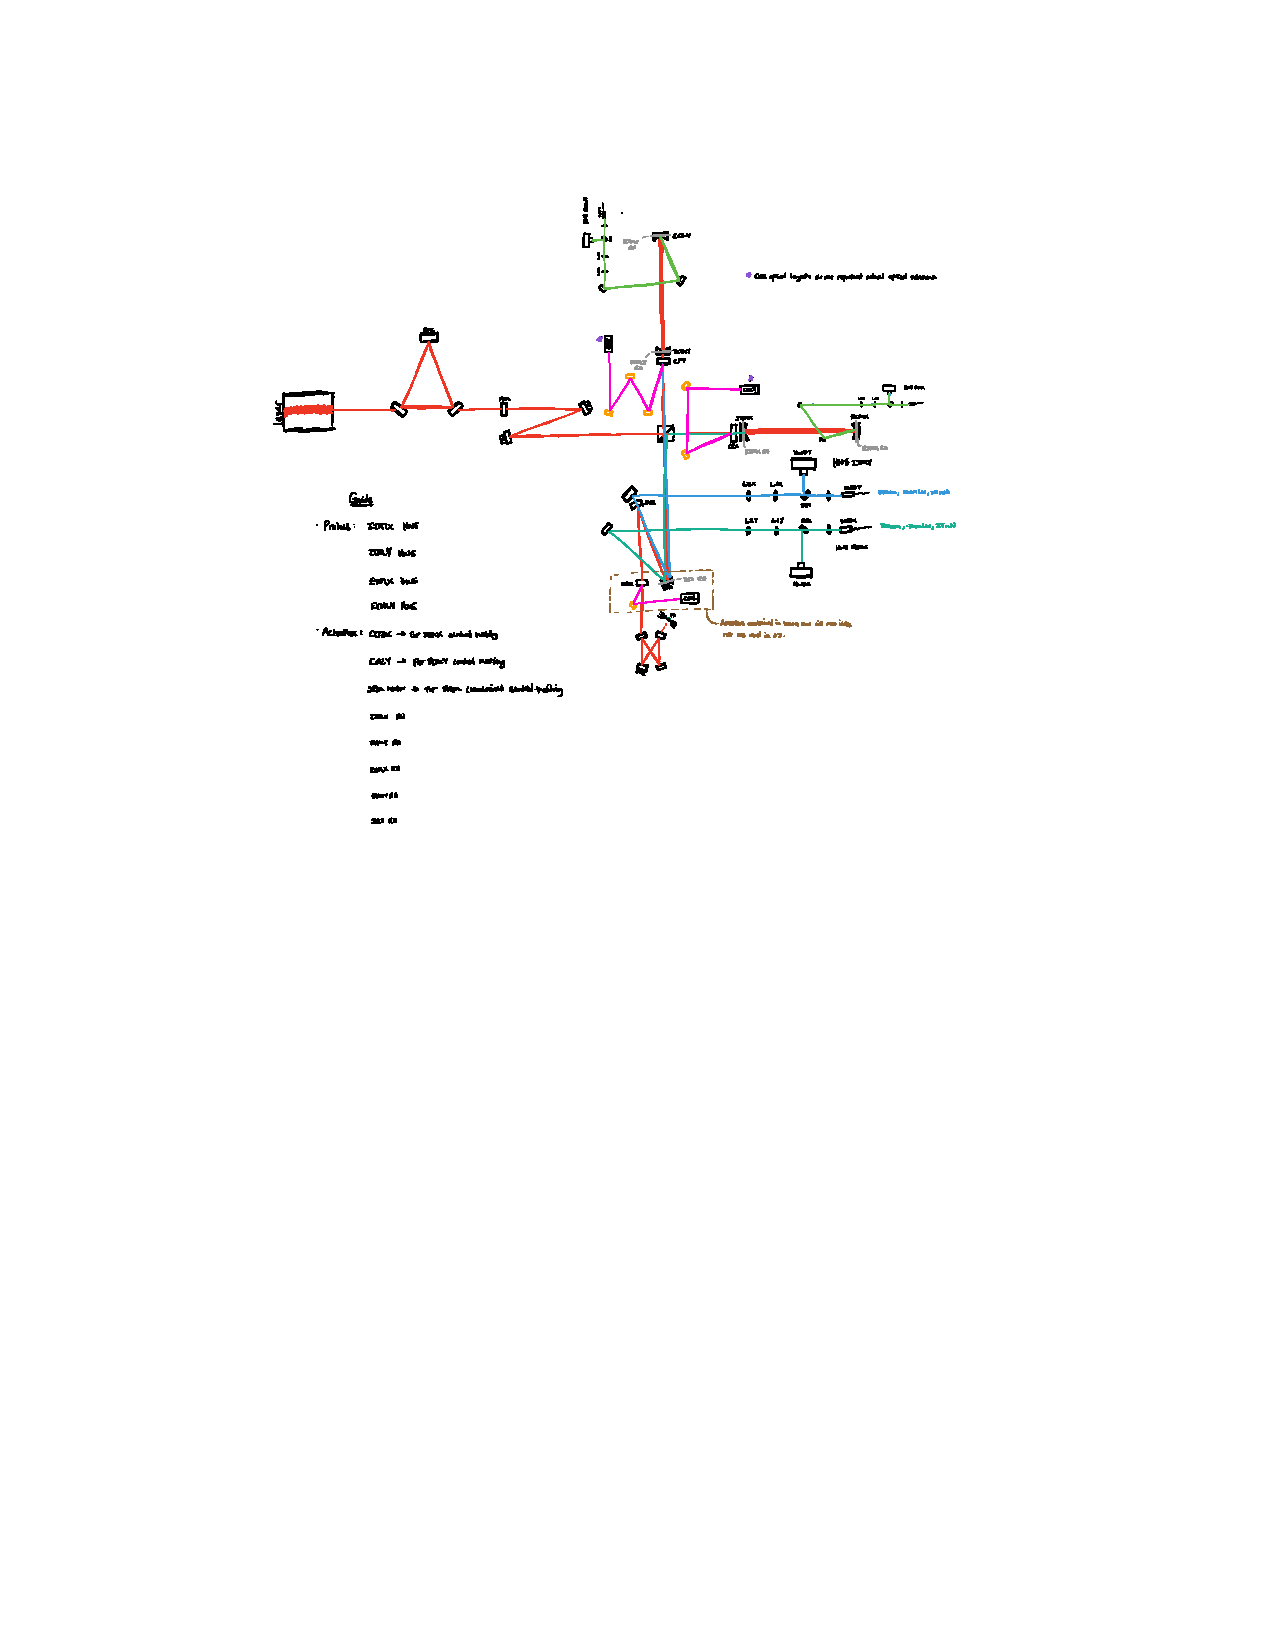
\includegraphics[width=1\textwidth=1]{TCS_schema_smaller.pdf}
        \caption{Cartoon figure (where can I get real one?)}
\end{figure}
    

\section{Measurements}
	\subsection{Differential Lens tuning}
		%% contrast defect %%

\subsubsection{Simple Michelson}
When handling and preparing your interferometer in a cold state you want to make sure you are minimizing your contrast. We define contrast as the following: 

$$ 
\mathrm{CD} = \frac{{\mid E_{\mathrm{ITMX}}-E_{\mathrm{ITMY}}\mid}^2}{{\mid E_{\mathrm{ITMX}}+E_{\mathrm{ITMY}}\mid}^2}
$$ 
Where $E_\mathrm{ITMX}$ and $E_\mathrm{ITMY}$ are the fields coming from ITMX and ITMY respectively. 

We measured this early to be ?
With the current TCS settings we measure it to be: 


\subsubsection{Locked DRFPMI}
Ideally, at lower arm power you would expect nearly the same mode shapes impinging from the arms onto the beamsplitter after the carrier has traveled through the arms. This is not the case with the finite absorption of the ITMs (bulk and surface) and ETMs (surface) which is guaranteed to introduce contrast with different absorption. Can tune your DARM offset so that you can understand what your contrast is in this configuration?

\subsubsection{Reducing Intensity and Frequency noise}


	\subsection{Absorption estimates}
		%% absorption estimates %%
\centering
    
        \begin{tabular}{ |p{1.5cm}|p{1.5cm}|p{1.5cm}|p{1.5cm}| }
        \hline
        ITMX & ETMX* & ITMY* & ETMY \\
        $.344\cdot10^{-6}$ & $.4\cdot10^{-6}$ & $.804\cdot10^{-6}$ & $.4\cdot10^{-6}$\\
        \hline
        \end{tabular}
 \begin{outline}
    \1 The arm gain 
        \2 Use result from \href{https://alog.ligo-wa.caltech.edu/aLOG/index.php?callRep=46683}{Craig's SRCL dither measurement}
    \1 Follow up with notes (uncertainties, potential point absorber issues.. maybe mention later)
    \1 Dan's idea of quantifying the absorption from integrating the OPD. Can we convert into an absorbed power?
 \end{outline}
	\subsection{Mode-matching}
		%% Mode matching %%

\subsection{RCs to arms}
\begin{itemize}
	\item Monitoring PRG and arm cavity buildups
\end{itemize}


\subsubsection{Arms to OMC}
\begin{itemize}
    \item Testing SR3 heating
        \subitem \href{https://alog.ligo-wa.caltech.edu/aLOG/index.php?callRep=46540}{alog 46540}
        \subitem NEEDS ANOTHER TEST
\end{itemize}
	\subsection{LHO locking with TCS}
		 %% TCS locking philosophy %%
 
 \begin{itemize}
    \item TCS actuation from 2 W to 50 W (what the models suggest), TVo model 

\begin{figure}[H]
        \centering
            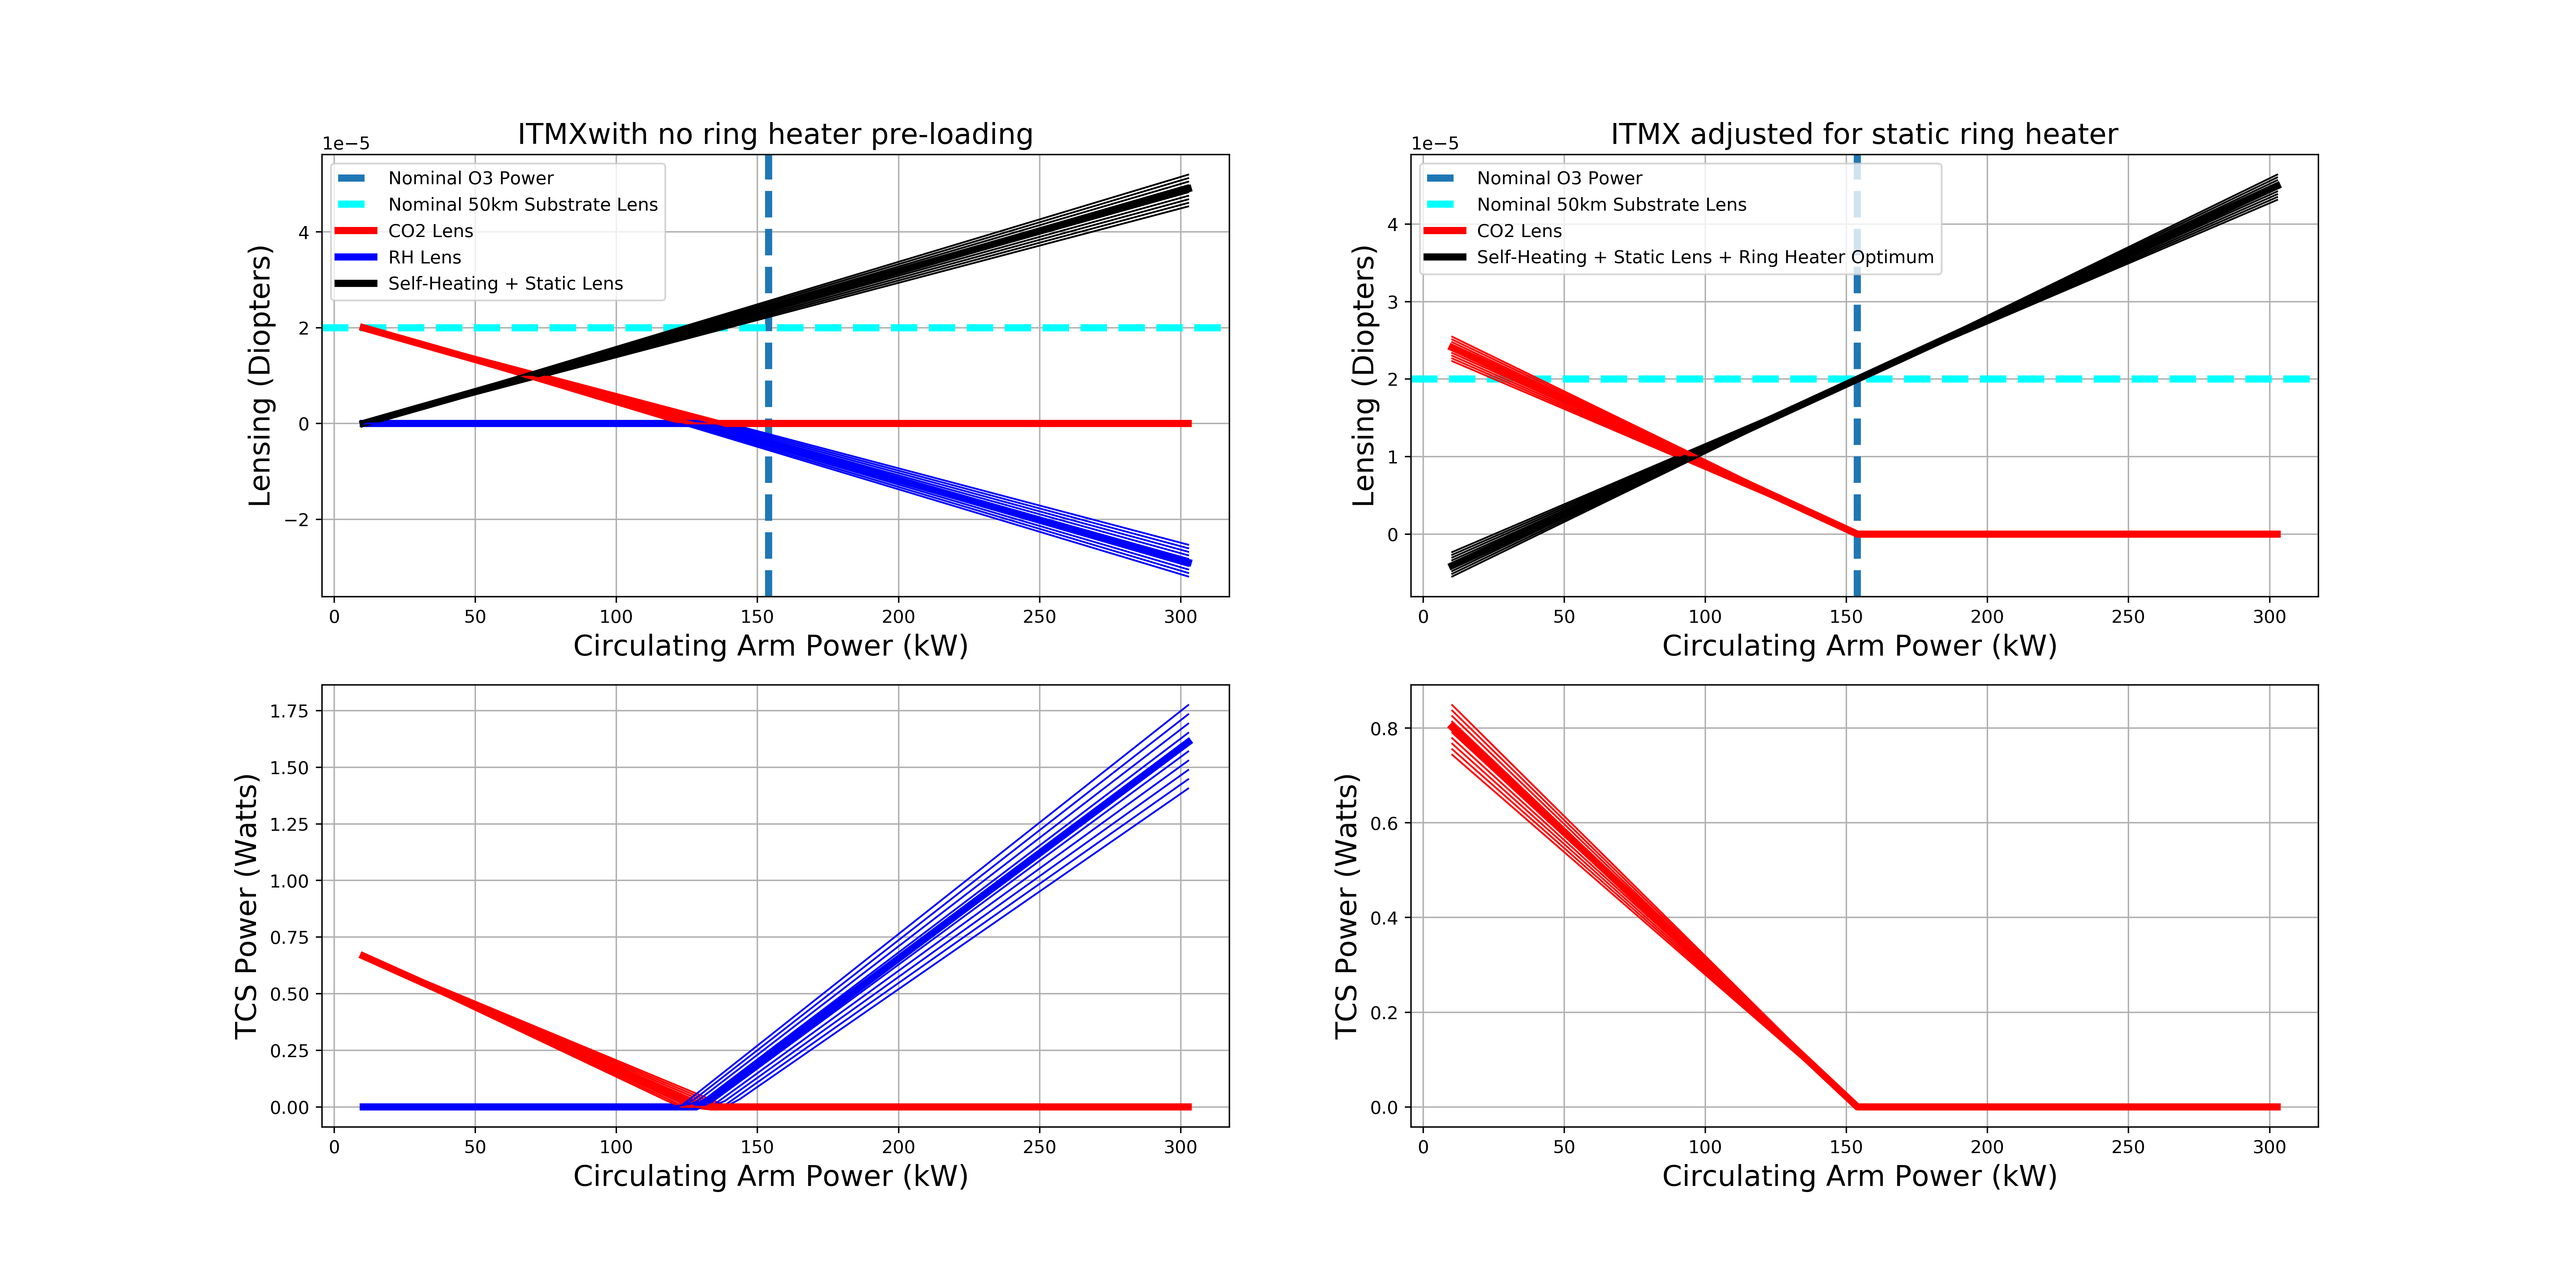
\includegraphics[width=1\textwidth]{ITMX_TCS_Settings.png}
            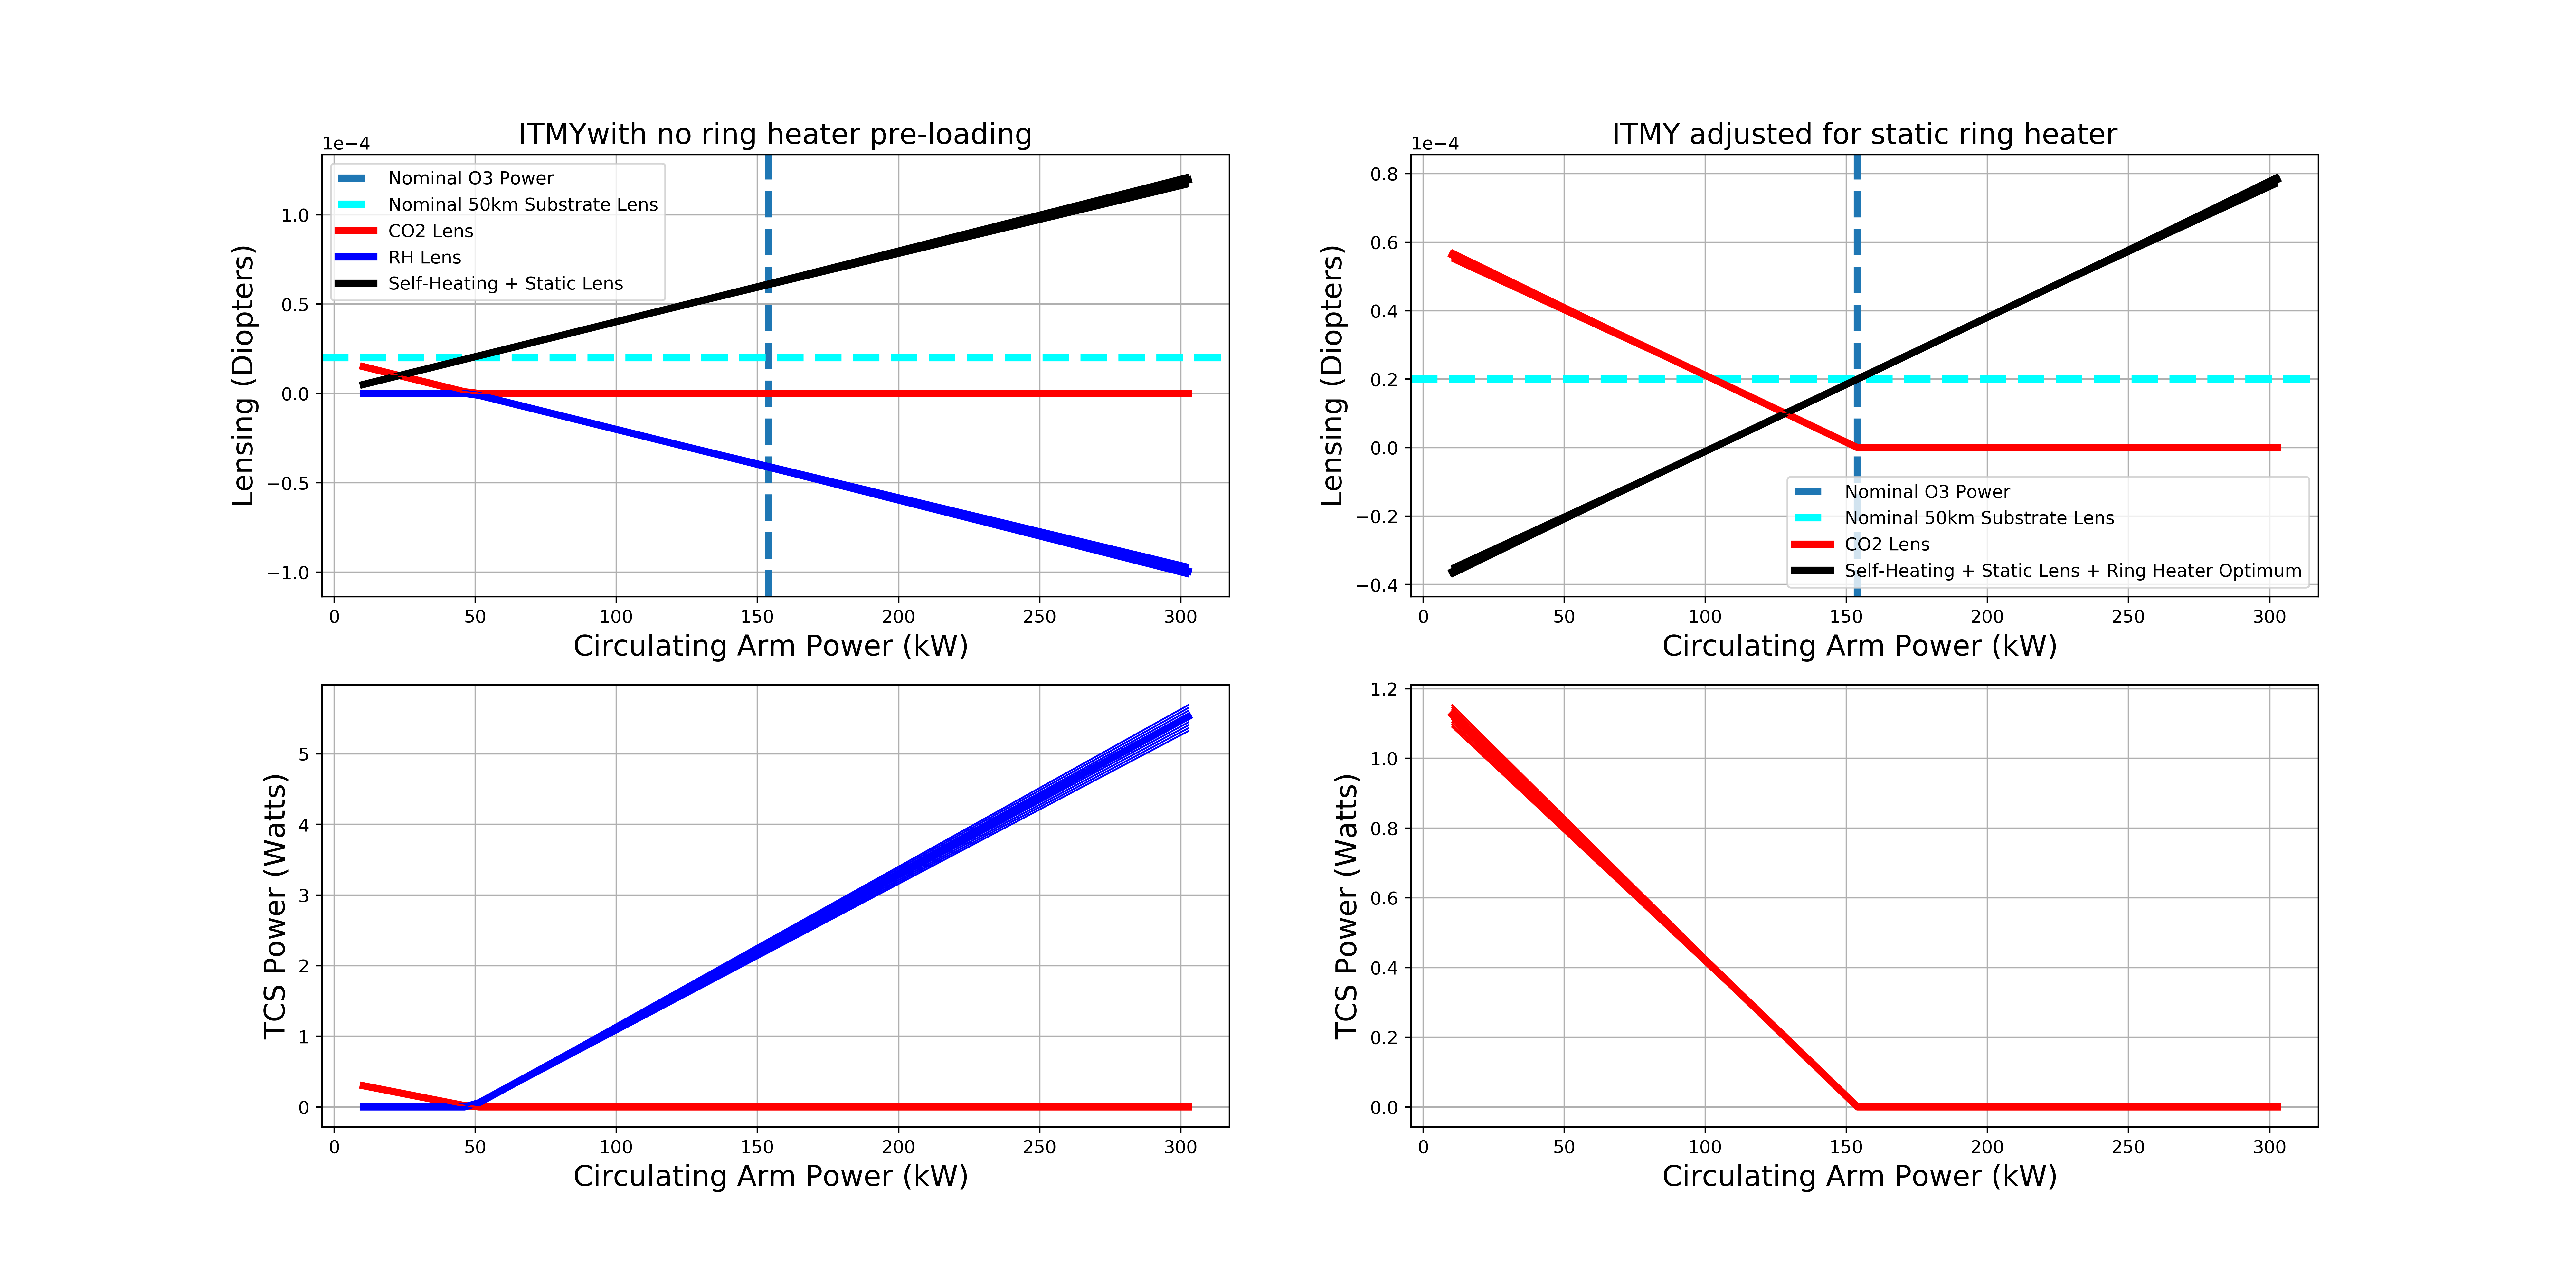
\includegraphics[width=1\textwidth]{ITMY_TCS_Settings.png}
            \caption{These plots assume that there are no high frequency spatial defects. PRG = 45, Arm gain = 228. Absorbed power for each test mass (in measurements) section. PC: Thomas Vo}
\end{figure}
    \item We separate TCS into two different states in the locking scheme while we attempt to achieve high power (assume we mean $\mathrm{P}_{\mathrm{in}} > 2 \mathrm{W}$): Preloading and High power operation. 

    \item Preloading
        \subitem The principle behind this state is to replicate the positive lens thermal distortions induced by a high power buildup within the interferometer arms and to properly compensate with the ring heaters to achieve an overall 50 km nominal lens. 
            \subsubitem Positive lens thermal distortions are replicated with CO2 lasers on the ITMX and ITMY compensation plates. 
        \subitem Allows for realistic commissioning of the interferometer controls in a "high power" thermal state.

    \item High power operation
        \subitem This state is achieved when increasing the input laser power (above 2 W) to a locked interferometer. 

\end{itemize}
     
	\subsection{Effects of high frequency spatial defects on test masses (Point absorbers)}
		%% point absorbers %%

 \begin{outline}
    \1 ITM point absorbers
     \begin{figure}[H]
            \centering
            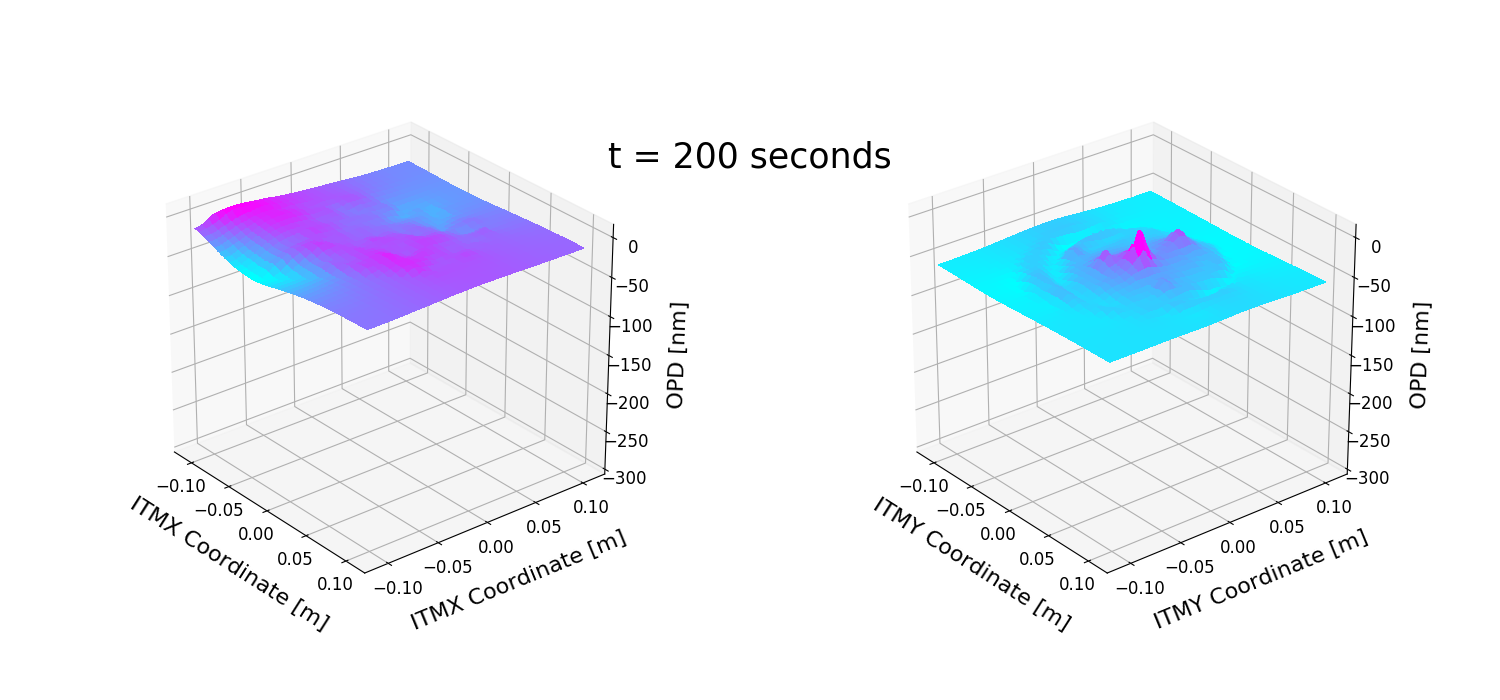
\includegraphics[width=.6\textwidth]{1231726400_3d_200dur_30W_ITM.png}
            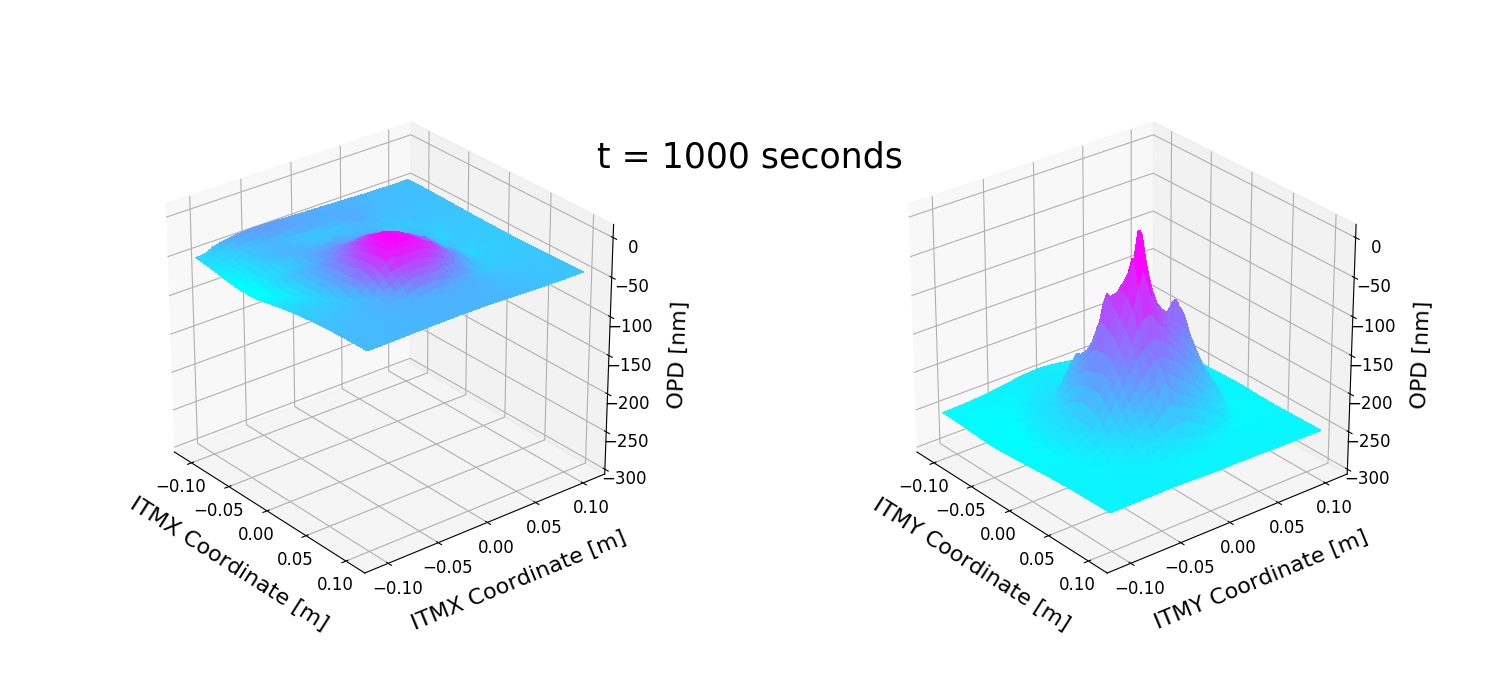
\includegraphics[width=.6\textwidth]{1231726400_3d_1000dur_30W_ITM.png}
            \caption{Comparision between the ITMX and ITMY HWS. PC: Thomas Vo}
      \end{figure}
        
    \2 ETM point absorbers
        \3 \href{https://alog.ligo-wa.caltech.edu/aLOG/index.php?callRep=45727}{alog 45727}
        
        \3 \href{https://alog.ligo-wa.caltech.edu/aLOG/index.php?callRep=44952}{first post}
    \2 Hurts contrast see Figure 3
    \2 Fast reduction in PRG and sideband buildup when increasing power to ifo
        \3 Time constant measurements
        \3 Dan's finesse simulation (\href{https://dcc.ligo.org/DocDB/0158/G1900090/002/20190116_tcs_call.pdf}{G1900090})
    \2 Scattering of the carrier into higher order modes in the arm cavities
        \3 Hiro's model
            \4 \href{https://dcc.ligo.org/DocDB/0158/G1900257/001/G1900257-v1.pdf}{Scattering of arm power to (n+m) = 7} 
    \1 Mode matching of the carrier from the Power Recycling cavities to the arms
        \2 Gabriele's models
            \3 \href{https://alog.ligo-wa.caltech.edu/aLOG/index.php?callRep=47027}{9 MHz (n+m)=9 transmission}
        \2 Hiro's model
 \end{outline}

\section{TCS settings going into O3}
	%% TCS settings %% 

\begin{outline}
    \1 Preloading: 
    	\2 Lenses in cold state: 
    		\3 ITMX
    			\4 Nominal substrate lens: -1.712 microdiopters
    			\4 CO2: .65 W 
    			\4 RH: 0.8 W (-14.4 $\mu$diopters from double pass lens)
    			\4 Overall induced lensing: 
    		\3 ITMY
    			\4 Nominal substrate lens: -23.81 microdiopters
    			\4 CO2: .83 W 
    			\4 RH: 2.6 W (-46.8 $\mu$diopters from double pass lens)
    			\4 Overall induced lensing:
    		\3 ETMX
    			\4 Nominal "lens": 
    			\4 RH: 0.4 W (-7.2 $\mu$diopters from double pass lens)
    			\4 Overall induced lensing*:
    		\3 ETMY 
    			\4 Nominal "lens":
    			\4 RH: 0.4 W 
    			\4 Overall induced lensing*: (-7.2 $\mu$diopters from double pass lens)
\end{outline}

* as seen by the carrier


\section{Future tests/measurements/analysis}
	%% future %%

\begin{itemize}
    \item SR3 heating
        \subitem \href{https://alog.ligo-wa.caltech.edu/aLOG/index.php?callRep=46540}{Short-ish SR3 measurement}
    \item SRM heating
    	\subitem Issues aligning when interferometer is locked? (\href{https://alog.ligo-wa.caltech.edu/aLOG/index.php?callRep=47342}{alog 47342})
        \subitem To improve mode-matching from the ifo to the OMC.
        \subitem This reduction in optical loss would allow optimal squeezing 
    \item SR3 and SRM 
    	\subitem Might be worth exploring this actuation space when assuming two nearly optimal actuators. 
    \item ITMY CO2 mask 
        \subitem Potential increase in sideband buildup as we are increasing power 
            \subsubitem Increased optical gain for length and angular control loops
        \subitem Aidan's pitch \href{https://alog.ligo-wa.caltech.edu/aLOG/index.php?callRep=46127}{alog 46127}
        \subitem Aidan's mask design \href{https://alog.ligo-wa.caltech.edu/aLOG/index.php?callRep=46738}{alog 46738}
        \subitem Aidan's mask model \href{https://alog.ligo-wa.caltech.edu/aLOG/index.php?callRep=46976}{alog 46976}
        \subitem Mask test \href{https://alog.ligo-wa.caltech.edu/aLOG/index.php?callRep=47081}{alog 47081}
            \subsubitem Improves 9MHz RIN coupling. Is this limiting us though?
            \subsubitem Projecting this 9MHz RIN coupling in the noise budget
                
    \item Moving spot position (Jenne and Dan moves)
    	\subitem Moving away from the ITMY and ETMX point absorbers?
        \href{https://alog.ligo-wa.caltech.edu/aLOG/index.php?callRep=47101}{alog 47101}
        \subsubitem
        \href{https://alog.ligo-wa.caltech.edu/aLOG/index.php?callRep=47117}{alog 47117}
        \subsubitem
        
\end{itemize}




\end{document}
